%%%%%%%%%%%%%%%%%%%%%%%%%%%%%%  IEEEsample.tex
%%%%%%%%%%%%%%%%%%%%%%%%%%%%%%%%%%%%%%%%%
%%%%%%%%%%%%%%%%%%%%%%%    More information: see the header of IEEEtran.sty
%%%%%%%%%%%%%%%%%%%%%%%
%%%%%%%%%%%%%%%%%%%%%%%%%%%%%%%%%%%%%%%%%%%%%%%%%%%%%%%%%%%%%%%%%%%%%%%%%%%%%%%%
%%%%

\documentclass[10pt,twocolumn]{IEEEtran}
%\documentclass[conference]{IEEEtran}

%%%\IEEEoverridecommandlockouts


%% set page size to US letter
\special{papersize=8.5in,11in}
\setlength{\pdfpageheight}{\paperheight}
\setlength{\pdfpagewidth}{\paperwidth}

\usepackage{xspace}
%\newcommand{\Grobner}{Gr\"{o}bner\xspace}

\usepackage{algorithm}
\usepackage[noend]{algpseudocode}



%% \usepackage[vlined,boxed,ruled]{algorithm2e}
%% %%for algorithm2e package, label has to be following caption in the same line!!!
%% \renewcommand{\algorithmcfname}{ALGORITHM}
%%  \SetAlFnt{\small}
%%  \SetAlCapFnt{\small}
%%  \SetAlCapNameFnt{\small}
%%  \SetAlCapHSkip{0pt}
%%  \IncMargin{-\parindent}

%% %% \RequirePackage{times}
%%  \RequirePackage{algorithmic}
%%  \PassOptionsToPackage{boxed}{algorithm}
%%  \RequirePackage{algorithm}
%%  \RequirePackage{multicol}
%% \renewcommand{\algorithmicrequire}{\textbf{Inputs:}}
%% \renewcommand{\algorithmicensure}{\textbf{Outputs:}}
 \DeclareMathAlphabet{\mathtsl}{OT1}{ptm}{m}{sl}

%\def\BibTeX{{\rm B\kern-.05em{\sc i\kern-.025em b}\kern-.08em1
%    T\kern-.1667em\lower.7ex\hbox{E}\kern-.125emX}}

%\newtheorem{theorem}{Theorem}
%\newtheorem{lemma}{Lemma}
%\newtheorem{example}{Example}
%\newtheorem{corollary}{Corollary}

\RequirePackage{amssymb, mathptm}
\usepackage{amsbsy}
\usepackage{amsthm}
\usepackage{graphicx}
\usepackage{helvet}
\usepackage{enumerate}
\usepackage{amsmath}
\usepackage{amsfonts}
\usepackage{graphicx}
\usepackage{multirow}
\usepackage{subfig}
\usepackage{comment}
\usepackage{cases}
\usepackage{xcolor}
\usepackage{epstopdf}
\usepackage[normalem]{ulem}

%%indent in algorithm


%\setcounter{page}{1}


% New command for the table notes.
\def\tabnote#1{{\small{#1}}}

% New command for the line spacing.
\newcommand{\ls}[1]
    {\dimen0=\fontdimen6\the\font
     \lineskip=#1\dimen0
     \advance\lineskip.5\fontdimen5\the\font
     \advance\lineskip-\dimen0
     \lineskiplimit=.9\lineskip
     \baselineskip=\lineskip
     \advance\baselineskip\dimen0
     \normallineskip\lineskip
     \normallineskiplimit\lineskiplimit
     \normalbaselineskip\baselineskip
     \ignorespaces
    }
%\renewcommand{\algorithmicrequire}{\textbf{Input:}}
%\renewcommand{\algorithmicensure}{\textbf{Output:}}

\newcommand{\beq}{\begin{equation}}
\newcommand{\eeq}{\end{equation}}
\newcommand{\beqarr}{\begin{eqnarray}}
\newcommand{\eeqarr}{\end{eqnarray}}
%\newcommand{\ov}{\overline}
\newcommand{\ov}{\bar}
\newcommand{\xor}{\bigoplus}
\newcommand{\Fm}{{\mathbb{F}}}
\newcommand{\myfontsize}{\fontsize{7}{9}\selectfont}


%the following is for space before and after align or other equation environment.

%%
\newtheorem{Algorithm}{Algorithm}[section]
\newtheorem{Definition}{Definition}[section]
\newtheorem{Example}{Example}[section]
\newtheorem{Proposition}{Proposition}[section]
\newtheorem{Lemma}{Lemma}[section]
\newtheorem{Theorem}{Theorem}[section]
\newtheorem{Corollary}{Corollary}[section]
\newtheorem{Conjecture}{Conjecture}[section]
\newtheorem{Problem}{Problem}[section]
\newtheorem{Notation}{Notation}[section]
\newtheorem{Setup}{Problem Setup}[section]

%%%

%%set spacing between table columns
\setlength{\tabcolsep}{3pt}

\begin{document}

%\thispagestyle{empty}
%\pagestyle{empty}

%\ls{1.5}


\title{\Large\textsc{Boolean Gr\"obner Basis Reductions on Datapath Circuits using the Unate Cube Set Algebra}}
\author{Utkarsh Gupta, Priyank Kalla, Vikas Rao \\
Electrical \& Computer Engineering, University of Utah \vspace{-0.2in}
}
%\affiliation{Electrical \& Computer Engineering, University of Utah}
% \email{}    
 
 
\maketitle
\thispagestyle{empty}
% Modified by  K. Kobayashi \maketitle 

%\markboth{MS Proposal by Tim Pruss}{}
\newcommand{\Fq}{{\mathbb{F}}_{q}}
\newcommand{\Fkk}{{\mathbb{F}}_{2^k}}
\newcommand{\Zkk}{{\mathbb{Z}}_{2^k}}
\newcommand{\Ftwo}{{\mathbb{F}}_{2}}
\newcommand{\Fkkx}[1][x]{\ensuremath{\mathbb{F}}_{2^k}[#1]\xspace}
\newcommand{\Grobner}{Gr\"{o}bner\xspace}
\newcommand{\B}{{\mathbb{B}}}
\newcommand{\Z}{{\mathbb{Z}}}
\newcommand{\F}{{\mathbb{F}}}
\newcommand{\G}{{\mathcal{G}}}
\newcommand{\alert}[1]{\textcolor{red}{#1}}

\newcommand{\spec}{{\it Spec}\xspace\ \xspace}
%%%

\newcommand{\debug}[1]{\textcolor{gray}{[ #1 ]}}


%%%%%%%%%%%%%%%%%%%% Include your files here %%%%%%%%%%%%%%%%%%%%%
\begin{abstract}
Recent developments in formal datapath verification make efficient use 
of symbolic computer algebra algorithms for formal verification. The
circuit is modeled as a set of polynomials over Boolean (or
pseudo-Boolean) rings, and  Gr\"obner basis (GB) reductions are
performed over these polynomials to derive a canonical
representation. GB reductions of Boolean polynomials tend to cause
intermediate expression swell (term explosion problem) -- often making
the approach infeasible in a practical setting. To overcome these
problems,  this paper describes a logic synthesis analogue of GB
reductions over Boolean polynomials, using the unate cube set algebra
over characteristic sets. By representing Boolean polynomials as
characteristic sets using Zero-suppressed BDDs (ZBDDs), implicit
algorithms can be efficiently designed for GB-reduction on digital
circuits. We show that imposition of circuit-topology based monomial
orders on ZBDDs enables an implicit implementation of polynomial
division, canceling multiple monomials in one-step. 
%Other recent
%strategies of GB-reduction on circuits can also be implemented
%efficiently on ZBDDs. 
Experiments performed over various finite field
arithmetic architectures demonstrate the efficiency of our 
algorithms and implementations as compared to conventional explicit
methods. 
\end{abstract}

\section{Introduction}

Craig interpolation is a method to construct and refine abstractions
of functions. It finds application in formal verification of hardware
designs and software programs, in logic synthesis of Boolean
functions, and also as a tool in proof complexity theory. It is a
logical tool to extract concise explanations for the infeasibility of
a mutually inconsistent set of statements. Craig
\cite{craig-interpolate} showed that for a valid implication $A
\implies B$, where $A, B$ are first order formulae containing no free
variables, there is a formula $I$ such that $A \implies I$, $I
\implies B$ and the non-logical symbols of $I$ appear in both $A$ and
$B$. The formula $I$ is called the {\it Craig interpolant}, or
interpolant for short. As  
propositional logic also admits Craig interpolation, the formal
verification community has extensively investigated interpolants and
their computation from resolution proofs of CNF-SAT problems. In the
propositional logic domain, the concept is stated with a slight
modification.  

\begin{Definition}\label{def:ci}
Let $(A, B)$ be a pair of CNF formulae (sets of clauses) such that $A
\w B$ is unsatisfiable. Then there exists a formula $I$ such that: (i)
$A\implies I$; (ii) $I \w B$ is unsatisfiable; and (iii) $I$ refers
only to the common variables of $A$ and $B$, i.e. $Var(I) \subseteq
Var(A) \cap Var(B)$. The formula $I$ is called the {\bf interpolant}
of $(A,B)$. 
\end{Definition}

Given the pair $(A, B)$ and their refutation proof, a procedure called
the {\it interpolation system} constructs the interpolant in linear
time and space in the size of the proof \cite{McMillan:CAV03}. As the
abilities of SAT solvers for proof refutation have improved,
interpolants have been exploited as abstractions in various problems
that can be formulated as unsatisfiable instances, e.g. model checking
\cite{McMillan:CAV03}, logic synthesis \cite{roland:bidecomp},
etc. Their use as abstractions have also been replicated in other
(combinations of) theories \cite{McMillan:TACAS04}
\cite{Kapur:SIGSOFT06} \cite{Cimatti:TACAS08} \cite{Griggio:FMCAD11},
etc.  
%These concepts have been applied to various problems in
%automated reasoning. 
%; {\it e.g.} for the theory of linear
%inequality \cite{McMillan:TACAS04}, data-type theories
%\cite{Kapur:SIGSOFT06}, Linear arithmetic and difference logic
%\cite{Cimatti:TACAS08}, Bit-vector theories \cite{Griggio:FMCAD11},
%among others.  


In this paper, we introduce the notion of {\it Craig interpolants in
polynomial algebra over finite fields} ($\Fq$) of $q$ elements, where
$q = p^k$ is a prime power. Given a mutually inconsistent pair of sets
of polynomials with coefficients from $\Fq$ that have no common zeros,
we show that Nullstellensatz over finite fields admits
interpolation. We represent the sets $A, B$ (from Def. \ref{def:ci}) as
{varieties of corresponding ideals}, and prove the existence of
an interpolant for the pair $(A,B)$. In this setting, {\it interpolants
correspond to varieties} -- subsets of the $n$-dimensional affine
space $\Fq^n$ -- and are represented by polynomial ideals, more
precisely, by a {\it Gr\"obner basis of corresponding ideals.}

Intuitively, it should be apparent that polynomial algebra over finite
fields would admit Craig interpolation (a first order theory over
$\Fq$ definitely admits quantifier elimination \cite{gao:qe-gf-gb}).
However, our literature search for interpolants and their computation
with polynomials in arbitrary finite fields did not reveal much prior
work in this area. %turned out to be unsuccessful. 
%There is a need for the theory and algorithms for
%interpolation in this domain. 
Recent years have witnessed
investigations in formal verification, abstraction and synthesis of
datapath circuits with $k$-bit operands, where the problems have been
modeled 
%using algebraic geometry 
over finite fields ($\Fkk$) \cite{pruss:tcad} \cite{xiaojun:hldvt2016}
or over finite integer rings ($\Zkk$) \cite{sivaram:todaes}. 
%Analogous to Boolean
%function decomposition, 
%there is also a need for polynomial (word-level) datapath synthesis
Interpolants can be exploited as abstractions of functions
($f:\Fkk\rightarrow\Fkk$) in this domain, and can make these
approaches practical. Motivated by the above needs, this paper
presents the theory of Craig interpolation in finite fields, and
describes algorithms to compute them.  


{\it Contributions:} Using the extensive machinery of algebraic
geometry in finite fields,
% -- including Nullstellensatz, projections of
%varieties, elimination and extension theory, set operations on ideals
%and varieties, etc. -- 
this paper makes the following contributions: 
1) Formally define the notion of interpolants in polynomial algebra
  over finite fields $\Fq$, and prove their existence in this domain.
2) Derive the relationship of interpolants with elimination ideals,
  and show how to compute them using Gr\"obner bases. 
3) Compute the {\it smallest} interpolant, i.e. the one
  contained in every other interpolant. Analogously, compute the
  {\it largest} interpolant, i.e. the one containing all
  other interpolants. 
4) Count the total number of all possible interpolants.
5) We show how all interpolants can be enumerated in
$\mathbb{F}_2$. However, as it is impractical to explore all possible
interpolants, we present an algorithm to heuristically enumerate a few
interpolants (explore the interpolant lattice): beginning with the
smallest, progressively visiting larger ones,   and terminating at the
largest interpolant.  

{\it Paper Organization:} The following section briefly reviews prior
work in Craig interpolation in various theories, and contrasts it
against the concepts presented in this paper. Section \ref{sec:prelim} 
describes the preliminary concepts of algebraic geometry and Gr\"obner
bases in finite fields. Section \ref{sec:theory} describes the theory
of interpolation in finite fields and shows how they can be computed
using the Gr\"obner basis algorithm. Section \ref{sec:alg} describes
techniques and an algorithm to enumerate the interpolants. 
%All the concepts are also demonstrated by means of
%examples. \debug{Section \ref{sec:dis} compares our results against
%interpolant-classification in propositional logic. --  we will see
%about this} 
Section \ref{sec:exp} describes some of our experiments with unsat
instances to generate the interpolants. Section
\ref{sec:conc} concludes the paper.  Some of the proofs of the
theorems and lemmas are omitted from the main body of the manuscript
and are included in an appendix. 

%The omitted proofs of
%the theorems and lemmas are contained in an appendix.

\vspace{-0.1in}
\section{Review of Previous Work}
In the past decade or so, there has been an explosion in the study,
classification and application of interpolants. In abstraction-based
model checking, interpolants are used as over-approximate image
operators \cite{McMillan:CAV03}. In Boolean function decomposition,
given a function $F(A, B, C)$ with support variables partitioned into
disjoint subsets $A, B, C$, it is required to decompose $F = G(A, C)
\odot H(B,C)$, where $\odot$ denotes the Boolean $\vee, \wedge,
\oplus$ operations. The existence of such a 
decomposition with the given variable partition is formulated as a
unsatisfiability checking problem. Craig interpolants can then be used
to compute $G, H$ \cite{roland:bidecomp}
\cite{roland:ashenhurst}. 
%Conceptually, these problems 
%have quantifiers and interpolants can be used in lieu of the more
%expensive quantifier elimination. 
In proof complexity, interpolants have been used as a tool to derive 
lower bounds; {\it e.g.} by reasoning that if $A\implies B$ does not
have a simple interpolant, then it cannot have a simple proof
\cite{pudlak:ci}. The authors in \cite{PudlakPCFA1998} present
an interpolation theorem for Nullstellensatz refutations and the
polynomial calculus \cite{CEI:stoc-96} which can then be used for
proving lower bounds. 

The use of interpolants as abstractions has also been replicated in
other combinations of theories. For example, the theory of linear
inequality \cite{McMillan:TACAS04}, data-type theories
\cite{Kapur:SIGSOFT06}, linear arithmetic and difference logic
\cite{Cimatti:TACAS08}, bit-vector SMT theories
\cite{Griggio:FMCAD11}, etc., are just a few of the many instances
of the usage of interpolation in various domains outside of purely
propositional logic. The aforementioned works derive interpolants from
resolution proofs obtained from SAT/SMT-solvers
(\cite{Cimatti:TACAS08}), or generate them by solving constrains
in the theories of linear arithmetic with uninterpreted functions
(\cite{Rybalchenko:VMCAI-2007}),  or exploit their connection to
quantifier elimination (\cite{Kapur:SIGSOFT06}), etc. As an 
alternative to interpolation, \cite{Kovacs2009} suggests the use of
local proofs and symbol eliminating inferences for invariant
generation.  
%%  to interpolation based on symbol
%% elimination inferences is presented in  which can be 
%% applied even for theories not having the interpolation property. 
However, the problem has been insufficiently investigated over
polynomial ideals in finite fields from an algebraic geometry
perspective. 


The works that come closest to ours are by Gao {\it et al.}
\cite{gao:qe-gf-gb} and \cite{gao:gf-gb-ms}. While they do not
address the interpolation problem per se, they do describe important
results of Nullstellensatz, projections of varieties and quantifier
elimination over finite fields that we extensively utilize in this
paper.  

The work of \cite{dsilva:vmcai2010} classifies (orders) the
interpolants according to their logical strength for model 
checking. They present a labeled interpolation system built on the
resolution proof where each vertex of the proof is annotated with
partially ordered labels.  Interpolants generated from different sets
of labels have the same  order of strength as the order of the labels.
This way a (sub-)lattice of interpolants is generated with the
smallest interpolant being the same as obtained from the McMillan's
system ($L_M$) \cite{McMillan:CAV03} and the largest being the
complement of inverse of $L_M$. In contrast, we present a method for
polynomials in $\F_2$ that can generate the complete lattice of
interpolants with the absolute smallest and   absolute largest
interpolants. The labeled interpolation system of
\cite{dsilva:vmcai2010} is generalized  to support  propositional
hyper-resolution proofs \cite{Weissenbacher2012}. 
% They show how to transform a refutation proof to generate
% interpolants of various strengths. 
More recently, \cite{rummer:fmcad2013} presents the notion of
interpolation abstraction, and describes a semantic framework for
exploring interpolant lattices. In contrast to these works that
qualitatively order the interpolants w.r.t. a given application
(e.g. model checking),  we describe a method to explore interpolants
based on the cardinality of the zero-sets of polynomial ideals, which
in turn corresponds to the size of the abstraction.  


\vspace{-0.1in}
\section{Notation and Preliminary Concepts}
\label{sec:prelim}
Let $\Fq$ denote the finite field of $q$ elements where $q=p^k$ is a
prime power, $\Fqbar$ be its algebraic closure, and $R = \fqring$ the
polynomial ring in $n$ variables $x_1,\dots,x_n$, with coefficients
from $\Fq$. A monomial is a power product of the form  $X =
x_1^{e_{1}}\cdot x_2^{e_{2}}\cdots x_n^{e_{n}}$, where  
$e_i \in \Z_{\geq 0}, i\in \{1, \dots,n\}$. A {\it polynomial} $f \in
R$ is written as a finite sum of terms   
$f = c_1 X_1 + c_2 X_2 + \dots + c_t X_t$, where $c_1, \dots, c_t$ are 
coefficients and $X_1, \dots, X_t$ are monomials. Impose a monomial
order $>$ (a term order) on the ring -- i.e. a total order and a
well-order on all the monomials of $R$ s.t. multiplication with
another monomial preserves the order. Then the monomials of all
polynomials $f = c_1 X_1 + c_2 X_2 + \dots + c_t X_t$ 
are ordered w.r.t. to $>$, such that  $X_1 > X_2 > \dots >  X_t$.
Subject to $>$, $lt(f) = c_1 X_1, ~lm(f) = X_1, ~lc(f) = c_1$,
are the {\it leading term}, {\it leading monomial} and {\it   leading
  coefficient} of $f$, respectively. In this work, 
we consider mostly with lexicographic (lex) term orders.

\subsubsection{Ideals, Varieties and Gr\"obner Bases:} 
Given a set of polynomials $F = \{f_1, \dots, f_s\}$ in $R$, the {\it
  ideal} $J \subseteq R$ generated by them is: %\vspace{-0.1in} 
$J = \langle f_1, \dots, f_s \rangle = \{\sum_{i=1}^{s} h_i\cdot f_i:
~h_i \in R\}.$ The polynomials $f_1, \dots, f_s$
form the {\it basis} or the {\it   generators} of $J$.    


Let $\bm{a} = (a_1,\dots,a_n) \in \Fq^n$ be a point in the affine
space, and $f$ a polynomial in $R$. If $f(\bm{a}) = 0$, we say
that $f$ {\it vanishes} on $\bm{a}$. We have to
analyze the {\it set of all common zeros} of the polynomials of $F$
that lie %$\{f_1, f_2,\dots, f_s\}$ 
within the field $\Fq$. This zero set is called the {\it variety}. It
depends not just on the given set of polynomials but rather on the
ideal generated by them. We denote it by $V_{\Fq}(J) =
V_{\Fq}(f_1,\dots,f_s)$, where: 
$$V_{\Fq}(J) = V_{\Fq}(f_1, \dots, f_s) = \{\bm{a} \in \Fq^n: \forall
f \in J, f(\bm{a}) = 0\}.$$

Varieties can be different when restricted to the given field $\Fq$
or considered over its algebraic closure $\Fqbar$. We will generally
drop the subscript when considering varieties over $\Fq$ and
denote $V(J)$ to imply $V_{\Fq}(J)$. The subscripts will be used,
however, to avoid any ambiguities, e.g. when comparing $V_{\Fq}(J)$
against the one over the closure $V_{\Fqbar}(J)$. 

Given two ideals $J_1 = \langle f_1,\dots,f_s\rangle, J_2=\langle
h_1,\dots,h_r\rangle$, the sum $J_1 + J_2 = \langle
f_1,\dots,f_s,h_1\dots,h_r\rangle$, and their product $J_1\cdot J_2 =
\langle f_i\cdot h_j: 1\leq i\leq s, 1\leq j\leq r\rangle$. Ideals and
varieties are dual concepts: $V(J_1 + J_2) = V(J_1) \cap V(J_2)$, and
$V(J_1\cdot J_2) = V(J_1) \cup V(J_2)$. Moreover, if $J_1 \subseteq
J_2$ then $V(J_1)\supseteq V(J_2)$.

%is an ideal, and so is their
%intersection $J_1\cap J_2$. 
%The union of ideals is, in general, not an
%ideal; however, $J_1 + J_2$ is the smallest ideal containing $J_1
%\cup J_2$. 



\underline{\it Gr\"obner Basis:} An ideal may have many different sets
of generators:  $J = \langle f_1,\dots,f_s\rangle = \dots = \langle
g_1,\dots,g_t\rangle$. Given a 
non-zero ideal $J$, a {\it Gr\"obner 
  basis} (GB) for $J$ is a finite set of polynomials $G = \{g_1,\dots,
g_t\}$ satisfying $\langle \{lm(f) ~|~ f \in J\} \rangle = \langle
lm(g_1),\dots,lm(g_t)\rangle$. Then $J = \langle G \rangle$ holds and
so $G=GB(J)$ forms a basis for $J$. A GB $G$ possesses important
properties that allow to solve many polynomial computation and
decision problems. The famous Buchberger's algorithm (see Alg. 1.7.1 
in \cite{gb_book}) takes as input the set of polynomials $F =
\{f_1,\dots,f_s\}$ and computes the GB
$G=\{g_1,\dots,g_t\}$. A GB can be {\it reduced} to eliminate
redundant polynomials from the basis. A reduced GB is a canonical
representation of the ideal. In this work, the set $G$ will denote a
reduced GB, and any reference to computation of an ideal can be 
construed as constructing its GB.  
%Also, when we reason about properties of ideals
%(interpolants), the reader may assume that a $G = GB(J)$ has been

\subsubsection{Varieties over finite fields and the structure of
  Gr\"obner bases:} When the variety of an ideal is finite, then the
ideal is said to be {\it zero-dimensional}. As $V_{\Fq}(J)$ is a
finite set, $J$ is zero-dimensional. 
%% As we operate over finite fields $\Fq$, which
%% are a finite set of points, we are concerned only with
%% zero-dimensional ideals.  
A GB for a zero dimensional ideal exhibits a 
special structure that we exploit in this work. 

For all elements $\alpha \in \Fq, \alpha^q = \alpha$. Therefore, the
polynomial $x^q-x$ vanishes everywhere in $\Fq$, and is called the
vanishing polynomial of the field, sometimes also referred to as the
field polynomial. Denote by $J_0 = \langle
x_1^q-x_1,\dots,x_n^q-x_n\rangle$ the ideal of all vanishing
polynomials in the ring $R$. Then $V_{\Fq}(J_0) = V_{\Fqbar}(J_0) =
\Fq^n$. Therefore, given any ideal $J$, $V_{\Fq}(J) = V_{\Fqbar}(J)
\cap\Fq^n = V_{\Fqbar}(J) \cap V_{\Fqbar}(J_0) = V_{\Fqbar}(J+J_0) =
V_{\Fq}(J+J_0)$. 



\begin{Theorem}[{\it The Weak Nullstellensatz over finite fields (from
      Theorem 3.3 in \cite{gao:gf-gb-ms})}]
\label{thm:weak-ns-ff}
{\it For a finite field $\Fq$ and the ring $R = \Fq[x_1, \dots, x_n]$, let
$J = \langle f_1, \dots, f_s\rangle \subseteq R$, and let $J_0 = \langle
x_1^q-x_1, \dots, x_n^q -  x_n\rangle$ be the ideal of vanishing
polynomials. Then $V_{\Fq}(J) = \emptyset \iff 1 \in J + J_0 \iff G =
reducedGB(J+J_0) = \{1\}$. }
\end{Theorem}

To find whether a set of polynomials $f_1,\dots,f_s$ have no common
zeros in $\Fq$, we can compute the reduced GB $G$ of
$\{f_1,\dots,f_s,x_1^q-x_1,\dots,x_n^q-x_n\}$ and see if $G = \{1\}$. If
$G\neq\{1\}$, then $f_1,\dots,f_s$ do have common zeros in $\Fq$, and
$G$ consists of the finite set of polynomials $\{g_1,\dots,g_t\}$ with the
following properties. 

\begin{Theorem}[{\it Gr\"obner bases in finite fields (application of
      Theorem 2.2.7 from \cite{gb_book} over $\Fq$)}]
\label{thm:gb-finite}
{\it For $G = GB(J+J_0) = \{g_1,\dots,g_t\}$, the following statements
  are equivalent:
\begin{enumerate}
\item The variety $V_{\Fq}(J)$ is finite.
\item For each $i = 1,\dots, n$, there exists some
$j\in\{1,\dots,t\}$ such that $lm(g_j) = x_i^l$ for some $l\in
\mathbb{N}$. 
\item The quotient ring ${\Fq[x_1\dots,x_n]}\over{\langle G\rangle}$ forms a
  finite dimensional vector space.
\end{enumerate}
}
\end{Theorem}

In other words, the ideal $J+J_0$ is zero-dimensional, and for each
variable $x_i$, there exists an element in the GB whose leading term
is a pure power of $x_i$. When that happens, we can also count the
number of solutions. For a GB $G$, let $LM(G)$ denote the set of 
 leading monomials of all elements of $G$: $LM(G) =
 \{lm(g_1),\dots,lm(g_t)\}$.  

\begin{Definition}[{\it Standard Monomials}]
Let $\bm{X^e} = x_1^{e_1}\cdots x_n^{e_n}$ denote a monomial. The set
of standard monomials of $G$ is defined as 
$ SM(G) = \{\bm{X^e} : \bm{X^e} \notin \langle LM(G) \rangle\}.$
\end{Definition}

\begin{Theorem}[{\it Counting the number of solutions (Theorem 3.7 in
      \cite{gao:gf-gb-ms})}] 
\label{thm:count}
{\it
Let $G = GB(J+J_0)$, and $|SM(G)| = m$, then the ideal $J$ vanishes on
$m$ distinct points in $\Fq^n$. In other words, $|V(J)| = |SM(G)|.$
}
\end{Theorem}

%% We demonstrate the application of these results using an example.

%% \begin{Example}
%% Consider the ideal $J_A = \langle ab, bd, bc + c, cd, bd + b + d + 1
%% \rangle \subset \F_2[a,b,c,d]$ and $J_0 = \langle a^2 - a,b^2 - b,c^2
%% - c,d^2 -d \rangle$. Using a lex term order with $a > e > b > c > d$,
%% compute $G = GB(J+J_0) = \{cd, b+d+1 \}

%% \end{Example}
%\include{exm1}

\subsection{Radical ideals and the Strong Nullstellensatz} 
\begin{Definition}
Given an ideal $J\subset R$ and $V(J) \subseteq \Fq^n$, the {\it ideal
of polynomials that vanish on} $V(J)$ is $I(V(J)) = \{ f \in R :
\forall \bm{a} \in V(J), f(\bm{a}) = 0\}$.
\end{Definition}

If $I_1 \subset I_2$ are ideals then $V(I_1) \supset V(I_2)$, and
similarly if $V_1 \subset V_2$ are varieties, then $I(V_1) \supset
I(V_2)$. 

\begin{Definition}
For any ideal $J\subset R$, the {\bf radical} of $J$ is defined
as $\sqrt{J} = \{f \in R: \exists m \in \mathbb{N} s.t. f^m \in J\}.$
\end{Definition}

When $J = \sqrt{J}$, $J$ is called a radical ideal. Over algebraically
closed fields, the {\it Strong Nullstellensatz} establishes the
correspondence between radical ideals and varieties. Over finite
fields, it has a special form. 


\begin{Lemma}
\label{lemma:radical-ff}
(From \cite{gao:qe-gf-gb}) For an arbitrary ideal $J\subset
\Fq[x_1,\dots,x_n]$, and  $J_0 = \langle
x_1^q-x_1,\dots,x_n^q-x_n\rangle$, the ideal $J + J_0$ is radical; 
i.e. $\sqrt{J+J_0} = J+J_0$. 
\end{Lemma}


\begin{Theorem}[{\it The Strong Nullstellensatz over finite fields
   (Theorem 3.2 in \cite{gao:qe-gf-gb})}] \label{thm:strong-ns}  
For any ideal $J \subset \Fq[x_1,\dots,x_n], ~I(V_{\Fq}(J)) = J + J_0$.
\end{Theorem}

%% \begin{proof}
%% $I(V(J)) = I(V_{\Fq}(J))  = I(V_{\Fqbar}(J + J_0) = \sqrt{J+J_0} = J + J_0$.
%% \end{proof}

\subsection{Projection of varieties and elimination ideals in finite
  fields} 

\begin{Definition}
Given an ideal $J = \langle f_1,\dots, f_s \rangle \subset R$ and its
variety $V(J) \subset \Fq^n$,  
the $l$-th projection of $V(J)$ denoted as $Pr_l(V(J))$ is the mapping
\begin{center}
$Pr_l(V(J)):\Fq^n \rightarrow \Fq^{n-l}, ~Pr_l(a_1,\dots,a_n) = (a_{l+1},\dots,a_n) $
\end{center}
for every $\bm{a} = (a_1,\dots,a_n) \in V(J)$.
\end{Definition}
% The projection of variety of $J_A$ from Example \ref{example:ja} on
% the variable set $C$ is $Pr_A(\Vac(J_A))$ and is equal to $(bcd):\{100,110,001\}$.

\begin{Definition}
Given an ideal $J \subset \Fq[x_1,\dots,x_n]$, the $l$-th elimination
ideal $J_l$ is an ideal in $R$ defined as $J_l = J \cap \Fq[x_{l+1},\dots,x_n]$.
\end{Definition}

The next theorem shows how we can obtain the generators of the $l$-th
elimination ideal using Gr\"obner bases.

\begin{Theorem}[{\it Elimination Theorem \cite{ideals:book}}]
Given an ideal $J \subset R$ and its GB $G$ $w.r.t.$ the
lexicographical (lex) order on the variables 
where $x_1 > x_2 > \cdots > x_n$, then for every $0 \leq l \leq n$ we
denote by $G_l$ the GB of $l$-th elimination ideal of $J$ and compute it as:
\begin{center}
$G_l = G \cap \Fq[x_{l+1},\dots,x_n]$
\end{center}
\end{Theorem}
% The elimination ideal corresponding to $J_A$ from Example \ref{example:ja}
% that eliminates the variables from the set $A$ is 
% $\langle cd,b+d+1 \rangle$ and its variety $\{001,100,110\}$.

In a general setting, the projection of a variety is a subset of the
variety of an elimination ideal: $Pr_l(V(J)) \subseteq V(J_l)$. However,
operating over finite fields, when the ideals contain the vanishing
polynomials, then the above set inclusion turns into an equality.


\begin{Lemma}[Lemma 3.4 in \cite{gao:qe-gf-gb}]
\label{lemma:project}
Given an ideal $J \subset R$ that contains the vanishing polynomials of 
the field, then $Pr_l(V(J)) = V(J_l)$, 
i.e. the $l$-th projection of the variety of ideal $J$ is equal to 
the variety of its $l$-th elimination ideal.

\end{Lemma}

%% \begin{Theorem}[Extension Theorem \cite{coxbook}] 
%% Given the ideal $J \in R$ and its first elimination ideal $J_1$,
%% write each generator $f_i (1\leq i\leq s)$ of $J$ in the form,
%% \begin{center}
%% $f_i = h_i(x_2,\dots,x_n)\cdot x_1^{N_i} + \text{monomials with degree of $x_1 < N_i$}$,
%% \end{center}
%% where $N_i \geq 0$ and $h_i \in \Fq[x_2,\dots,x_n]$ is non-zero. Let's say that there is
%% point $(a_2,\dots,a_n)$ in $V(I_1)$. If $(a_2,\dots,a_n) \not \in V(h_1,\dots,h_s)$,
%% then there exists $a_1 \in \Fq$ such that 
%% $(a_1,a_2,\dots,a_n) \in V(J)$.   
%% \end{Theorem}

%% In other words, if the condition $(a_2,\dots,a_n) \not \in V(h_1,\dots,h_s)$ is satisfied,
%% then the point $(a_2,\dots,a_n) \in V(I_1)$ can be extended to a point
%% $(a_1,a_2,\dots,a_n) \in V(J)$.
%% \par For an ideal $J$ that contains the vanishing polynomials, its GB
%% $G = \{g_1,\dots,g_t\}$ has the property that for each variable in $\{x_1,\dots,x_n\}$
%% there must be some polynomial $g_i$ such that $lm(g_i) = x_i^l$ for $l \in \mathbb{N}$.
%% Therefore, every point in $V(G_l)$ can be extended to a point in $V(G)$.  

We will utilize all of the above concepts to derive the results in
this paper. 


\section{Theory}
\label{sec:theory}
We describe the setup for Craig interpolation in the ring
$R=\Fq[x_1,\dots,x_n]$. Partition the variables $\{x_1,\dots,x_n\}$
into disjoint subsets $A, B, C$. We are given two ideals $J_A \subset
\Fq[A,C], J_B \subset \Fq[B,C]$ such that the $C$-variables are common
to the generators of both $J_A, J_B$. {\it From here on, we will
  assume that all ideals include the corresponding vanishing
  polynomials.}  For example, generators of $J_A$ include $\bm{A^q -
A, C^q-C}$ where 
$\bm{A^q-A} = \{x_i^q - x_i: x_i \in A\}$, and so on. Then these
ideals become radicals and we can apply Lemmas \ref{lemma:radical-ff}
and \ref{lemma:project}. We use $\Vac(J_A)$ to denote the variety of
$J_A$ over the $\Fq$-space spanned by $A$ and $C$ variables, 
i.e. $\Vac(J_A) \subset \Fq^A \times \Fq^C$. Similarly,
$\Vbc(J_B)\subset\Fq^B\times\Fq^C$. 

Now let $J = J_A + J_B \subseteq \Fq[A,B,C]$, and suppose that it is
found by application of the Weak Nullstellensatz
(Thm. \ref{thm:weak-ns-ff}) that $\Vabc(J) = \emptyset$. When we
compare the varieties of $J_A$ and $J_B$, then we can consider the
varieties in $\Fq^A\times\Fq^B\times\Fq^C$,  as $\Vabc(J_A) =
\Vac(J_A) \times \Fq^B \subset \Fq^A\times\Fq^B\times\Fq^C$. With this
setup, we define the interpolants as follows.


\begin{Definition}[{\it Interpolants in finite fields}]
\label{def:int}
Given two ideals $J_A \subset \Fq[A,C]$ and $J_B \subset \Fq[B,C]$
where $A,B,C$ denote the three disjoint sets of variables such that 
$\Vabc(J_A) \cap \Vabc(J_B) = \emptyset$. Then there exists an ideal 
$J_I$ satisfying the following properties:
\begin{enumerate}
\item $\Vabc(J_I) \supseteq \Vabc(J_A)$
\item $\Vabc(J_I) \cap \Vabc(J_B) = \emptyset$
\item The generators of $J_I$ contain only the $C$-variables;
 or $J_I \subseteq \Fq[C]$.
\end{enumerate}
We call $\Vabc(J_I)$ the {\bf interpolant} in finite fields of the
pair $(\Vabc(J_A), \Vabc(J_B))$, and the corresponding ideal $J_I$ is
called the {\bf ideal-interpolant}. 
\end{Definition}

As the generators of $J_I$ contain only the $C$-variables, the
interpolant $\Vabc(J_I)$ is of the form $\Vabc(J_I) =
\Fq^A\times\Fq^B\times\Vc(J_I)$. 
%Before we prove the existence of
%$J_I$ and classify the other interpolants, we demonstrate the concept
%of interpolants and ideal-interpolants using an example. 


\begin{Example}
\label{ex:main}
{\it 
Consider the ring $R = \F_2[a, b, c, d,e]$, partition the variables as
% \begin{center}
 $A = \{a\}, B = \{e\}, C = \{b,c,d\}.$
% \end{center}
Let ideals 

\vspace{-0.2in} 

\begin{align*}
 J_A &= \langle ab, bd, bc + c,
 cd, bd + b + d + 1
 \rangle + J_{0,A,C}\\
 J_B &= \langle b,d,ec+e+c+1,
 ec
 \rangle + J_{0,B,C}
 \end{align*}

\vspace{-0.1in} 

where $J_{0,A,C}$ and $J_{0,B,C}$ are the corresponding ideals of vanishing
polynomials. Then, we have

\vspace{-0.2in} 

\begin{align*}
\Vabc(J_A) &= \Fq^B \times \Vac(J_A)  \\
&= (abcde):\{ 01000,00010,01100,10010, \\
& ~~~~~~~~~~~~~~~~~~~~~~ 01001,00011,01101,10011 \} \\
\Vabc(J_B) &= \Fq^A \times \Vbc(J_B) \\
&= (abcde):\{00001,00100,10001,10100\}
\end{align*} 

The ideals $J_A, J_B$ have no common zeros as $\Vabc(J_A) \cap
\Vabc(J_B) = \emptyset$.   
The pair $(J_A, J_B)$ admits a total of 8 interpolants:\\

\begin{minipage}[c]{0.5\textwidth}

{\small
\begin{enumerate}
\item $V(J_S) = (bcd): \{001,100,110\}$\\ 
% is the smallest interpolant,   with ideal-interpolant 
$J_S = \langle cd, b + d+ 1 \rangle$

\item  	 	$V(J_1) = (bcd): \{001,100,110,101\}$\\
$J_1 = \langle cd,bd+b+d+1,bc+cd+c \rangle$ 

\item 
 	$V(J_2) = (bcd): \{001,100,110,011\}$ \\
 	$J_2 = \langle b+d+1 \rangle$ 

\item 
 	$V(J_3) = (bcd): \{001,100,110,111\}$ \\
 	$J_3 = \langle b+cd+d+1 \rangle$ 

\item 
 	$V(J_4) = (bcd): \{001,100,110,011,111\}$ \\
 	$J_4 = \langle bd+b+d+1,bc+b+cd+c+d+1 \rangle$ 

\item 
 	$V(J_5) = (bcd): \{001,100,110,101,111\}$ \\
 	$J_5 = \langle bc+c,bd+b+d+1 \rangle$ 

\item 
 	$V(J_6) = (bcd): \{001,100,110,101,011\}$  \\
 	$J_6 = \langle bd+b+d+1,bc+cd+c \rangle$ 

\item $V(J_L) = (bcd): \{001,011,100,101,110,111\}$ \\
%is the largest  interpolant, with ideal 
$J_L = \langle bd + b + d + 1 \rangle$.

\end{enumerate}
}
\end{minipage}
\hspace{0.3cm}
\begin{minipage}{0.5\textwidth}
% \begin{figure}[hbt]
% \begin{center}
% \centering
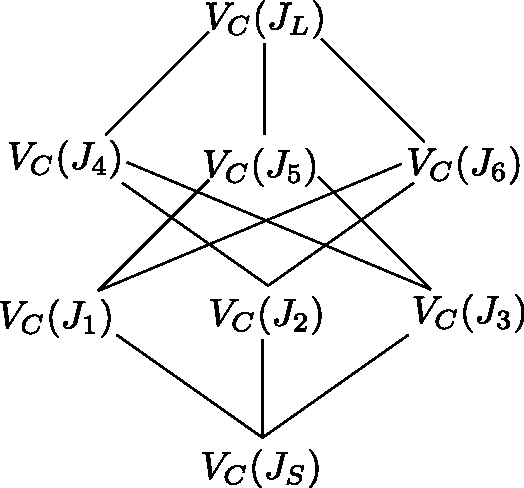
\includegraphics[width=0.8\textwidth]{interpolant_lattice.pdf}
\captionof{figure}{Interpolant lattice}
\label{Fig:int_lat}
% \begin{center}
% \end{figure}
\end{minipage}

It is easy to check  that all $V(J_I)$ satisfy the 3 conditions of
Def. \ref{def:int}. Note also that $V(J_S)$ is the smallest
interpolant, contained in every other interpolant. Likewise, $V(J_L)$
contains all other interpolants and it is the largest. The other
containment relationships are shown in the corresponding interpolant
lattice in Fig. \ref{Fig:int_lat}; i.e. $\Vc(J_1) \subset \Vc(J_5),
\Vc(J_1) \subset \Vc(J_6)$, and so on. 


 %% \begin{align*}
 %% & \Vc(J_1) \subset \Vc(J_5) ~~~~~~~~~~~~ \Vc(J_1) \subset \Vc(J_6) \\
 %% & \Vc(J_2) \subset \Vc(J_4) ~~~~~~~~~~~~ \Vc(J_2) \subset \Vc(J_6) \\
 %% & \Vc(J_3) \subset \Vc(J_4) ~~~~~~~~~~~~ \Vc(J_3) \subset \Vc(J_5)
 %% \end{align*}


}
\end{Example}



%% \begin{Example}
%% \label{example:jajb}
%% Consider the ideal $J_A$ from Example \ref{example:ja} and another
%% $J_B = \langle b,d,ec+e+c+1, ec \rangle$ with the variables of 
%% its generators partitioned as $B = \{e\}$ and $C = \{b,c,d\}$.
%% The intersection of varieties $\Vabc(J_A)$ and $\Vabc(J_B)$ is 
%% empty as,
%% \begin{align*}
%% \Vabc(J_A) &= \Fq^B \times \Vac(J_A)  \\
%% &= (abcde):\{ 01000,00010,01100,10010, \\
%% & ~~~~~~~~~~~~~~~~~~~~~~ 01001,00011,01101,10011 \} \\
%% \Vabc(J_B) &= \Fq^A \times \Vbc(J_B) \\
%% &= (abcde):\{00001,00100,10001,10100\}
%% \end{align*} 

%% Therefore, there must exist an interpolant satisfying the 
%% above three properties. 
%% \end{Example}


\begin{Theorem}
An ideal-interpolant $J_I$, and correspondingly the interpolant $\Vabc(J_I)$, as
given in Def. \ref{def:int}, always exists. 
\end{Theorem}

\begin{proof}
Consider the elimination ideal $J_I = J_A \cap \Fq[C]$. We show $J_I$ satisfies 
the three conditions for the interpolant. 

\par \noindent  \underline{Condition 1}: $\Vabc(J_I) \supseteq
\Vabc(J_A)$. This condition is trivially satisfied due  to
construction of elimination ideals. As $J_I \subseteq J_A$,
$\Vabc(J_I) \supseteq \Vabc(J_A)$.

%% In other words  any point in the $\Vabc(J_A)$ has
%% to satisfy all the polynomials in $J_I$ as $J_I$ is  a subset of
%% polynomials in $J_A$.  

\par \noindent \underline{Condition 2}: $\Vabc(J_I) \cap \Vabc(J_B) =
\emptyset$. This condition  can be equivalently stated as $\Vbc(J_I)
\cap \Vbc(J_B) = \emptyset$ as neither  $J_I$ nor $J_B$ contains any
variables from the set $A$. We prove this condition by
contradiction. Let's assume that there exists a
common point $(\mathbf{b},\mathbf{c})$ in $\Vbc(J_I)$ and $\Vbc(J_B)$.  
We know that the projection of the variety $Pr_A(\Vac(J_A))$ is equal
to the variety of the elimination ideal $\Vc(J_I)$, where $J_I=J_A
\cap \Fq[C]$, due to Lemma \ref{lemma:project}. 
 %% (as $J_A$ is radical). 
Therefore, the point $(\mathbf{c})$ in the variety of $J_I$ can be
extended to a point $(\mathbf{a},\mathbf{c})$ in the variety of
$J_A$. This implies that the ideals $J_A$ and $J_B$ vanish at 
($\mathbf{a},\mathbf{b},\mathbf{c}$). This is a contradiction to our
initial assumption that the intersection of the varieties of $J_A$ and
$J_B$ is empty.  Thus $J_I, J_B$ have no common zeros.

\par \noindent \underline{Condition 3}: The generators of $J_I$
contain only the $C$-variables. This condition is trivially satisfied
as $J_I$ is the elimination ideal obtained by  eliminating
$A$-variables in $J_A$. 
\end{proof}

The above theorem not only proves the existence of an interpolant, but
also gives a procedure to construct one: $J_I = J_A\cap\Fq[C]$. In
other words, compute a reduced Gr\"obner basis $G$ of $J_A$ w.r.t. an
elimination order $A> B > C$ and take $G_I = G \cap \Fq[C]$. Then
$G_I$ gives the generators for the ideal-interpolant $J_I$.

\begin{Example}
{\it 
The elimination ideal $J_I$ computed for $J_A$ from Example \ref{ex:main}
is $J_I = J_S = \langle cd,b+d+1 \rangle$ with variety
$\Vc(J_I)=(bcd):\{001,100,110\}$.  This variety over the variable set
$A$ and $C$ is $\Vac(J_I)=(abcd):\{0001,0100,0110, 1001,1100,1110\}$,
and it contains $\Vac(J_A)$. Moreover, $\Vabc(J_I)$ also has an empty
intersection with $\Vabc(J_B)$. 
}
\end{Example}

%The next theorem proves that this variety $\Vc(J_I)$ is also the
%smallest interpolant, $i.e.$ all other interpolants contain it. 

\begin{Theorem}
\label{thm:smallest}
The interpolant $\Vabc(J_S)$ corresponding to the ideal %-interpolant
$J_S = J_A \cap \Fq[C]$ is the smallest interpolant.
\end{Theorem}

\begin{proof} 
The proof is given in the appendix. 


%% Let $J_I \subseteq \Fq[C]$ be any another ideal-interpolant $\neq
%% J_S$. We show that $\Vc(J_S) \subseteq \Vc(J_I)$. For $\Vc(J_I)$
%% to be an interpolant it must satisfy 
%% \begin{align*}
%% \Vabc(J_A) \subseteq \Vabc(J_I)
%% \end{align*}
%% which is equivalent to 
%% \begin{align*}
%% I(\Vabc(J_A)) &\supseteq I(\Vabc(J_I)) \\
%% \implies J_A &\supseteq J_I  
%% \end{align*}
%% due to Theorem \ref{thm:strong-ns}.
%% %% as $J_I$ is radical so $I(\Vabc(J_I)) = J_I)$. 
%% As the generators of $J_I$ only contain polynomials in $C$-variables,
%% this relation also holds for the following
%% \begin{align*}
%% J_A \cap \Fq[C] &\supseteq J_I \\
%% \implies J_S &\supseteq J_I \\
%% \implies \Vc(J_S) &\subseteq \Vc(J_I).
%% \end{align*} 
\end{proof}

%After proving that the elimination ideal $J_A \cap \Fq[C]$ is the
%smallest interpolant, 
Now we discuss how the largest interpolant can be
computed. For this, we will make use of quotients of ideals. 

\begin{Definition}
\label{def:quo}
({Quotient of Ideals}) If $J_1$ and $J_2$ are ideals in a ring $R$,
then $J_1:J_2$ is the set 
%  \begin{equation}
  $\{f \in R \ |\ f\cdot g \in J_1, \forall g \in J_2\}$ %\nonumber
%  \end{equation}
and is called the {\bf ideal quotient} of $J_1$ by $J_2$.
\end{Definition}

We use ideal quotients to compute the complement of a variety. Given
an ideal $J' \subset R$ containing the vanishing polynomials, suppose
we need to find an ideal $J$ such that $V(J) = \Fq^n - V(J') = V(J_0)
- V(J')$, where ``$-$'' corresponds to the set difference
operation. Then $J = J_0 : J'$ (see Theorem III.2 and Corollary III.1
in \cite{xiaojun:hldvt2016} for a proof outline). Once again, the
Gr\"obner basis algorithm can be used to compute $J_0:J'$ 
\cite{ideals:book}.  

\begin{Theorem}
\label{thm:large}
Consider the elimination ideal $J'_L = J_B \cap \Fq[C]$. The
complement of the variety $\Vc(J'_L)$,  computed as $\Fq^C - \Vc(J'_L)$,
is the largest interpolant.
\end{Theorem}

\begin{proof} Proof is given in the appendix. 

%% We first prove that the interpolant computed by
%% complementing $\Vc(J'_L)$  as $\Fq^C - \Vc(J'_L)$ is indeed a valid
%% interpolant. As $J'_L$ is the elimination ideal computed from $J_B$,
%% $\Vbc(J'_L) \supseteq \Vbc(J_B)$. This in turn implies that the
%% complement of $V(J'_L)$ cannot intersect with $V(J_B)$ at any
%% point. This proves condition 2 for $\Fq^C - \Vc(J'_L)$ to be a
%% valid interpolant.  

%% For condition 1, we need to prove that
%% \begin{align*}
%% \Vac(J_A) \subseteq \Fq^A \times (\Fq^C - \Vc(J'_L))
%% \end{align*}
%% This can be restated as
%% \begin{align*}
%% \Vac(J_A) \cap \Fq^A \times \Vc(J'_L) = \emptyset
%% \end{align*}
%% Let us assume (by contradiction) that there exists a common point 
%% $(\mathbf{a},\mathbf{c})$ in $\Vac(J_A)$ and $\Fq^A \times
%% V_C(J'_L)$. As the projection $Pr_B(\Vbc(J_B))$ on the
%% $C$-variables is equal to  the variety of the elimination ideal
%% $\Vc(J'_L)$, a point $(\mathbf{c}) \in \Vc(J'_L)$ can be  extended to
%% some point $(\mathbf{b},\mathbf{c})$ in $\Vbc(J_B)$. This implies that
%% the point $(\mathbf{a},\mathbf{b},\mathbf{c})$ is a common point in
%% $\Vabc(J_A)$ and $\Vabc(J_B)$, which is a contradiction to our initial
%% assumption. Therefore condition 1 of Def. \ref{def:int} is satisfied
%% too and $\Fq^C - \Vc(J'_L)$ is indeed an interpolant. 

%% \par \noindent Next we prove that $\Fq^C - \Vc(J'_L)$ is the largest
%% interpolant. Consider an arbitrary ideal-interpolant $J_I$. We want to
%% prove $\Vc(J_I) \subseteq \Fq^C - \Vc(J'_L)$, or equivalently to prove
%% $\Vc(J_I) \cap \Vc(J'_L) = \emptyset$. Let us assume (by contradiction) 
%% that there exists a common point $(\mathbf{c})$ in $\Vc(J_I)$ and
%% $\Vc(J'_L)$. As $J'_L$ is the elimination ideal of $J_B$, this point
%% can be extended to some point $(\mathbf{b},\mathbf{c})$  
%% in $\Vbc(J_B)$. This in turn implies that $(\mathbf{b},\mathbf{c})$ is
%% a common point in  $\Vbc(J_B)$ and $\Fq^B \times \Vc(J_I)$. This is a
%% contradiction as an interpolant cannot intersect with the variety of
%% $J_B$. Hence, $\Fq^C - \Vc(J'_L)$ is the largest interpolant and it
%% contains all other interpolants.

\end{proof}

Let $J_L$ be the radical ideal corresponding to the largest
interpolant $\Vc(J_L) = \Fq^C - \Vc(J'_L)$. This ideal-interpolant
$J_L$ can be computed as $J_L = (J_{0,C}:J'_L)$, where $J_{0,C}$ is
ideal of vanishing polynomials in $C$-variables.  


\begin{Example}
{\it 
The ideal-interpolant $J_L = \langle bd + b + d + 1 \rangle$ in 
Example~\ref{ex:main} is computed as:
\begin{itemize}
	\item First compute the ideal $J'_L = J_B \cap \Fq[C]$ which results in 
	$J'_L = \langle b,d \rangle$.
	\item Then compute $J_L$ as $J_L = J_{0,C}: J'_L$ which results in
	$J_L = \langle bd + b + d + 1 \rangle$
\end{itemize}
The variety $V_C(J_L)=(bcd):\{001,011,100,101,110,111\}$ and it is the
largest interpolant for the given pair ($J_A,J_B$). 
}
\end{Example}

\begin{Lemma}
\label{noofinter}
The total number of interpolants for the pair ($J_A,J_B$) is
$2^{|SM(J_D)|}$, where $J_D = (J_L:J_S)$. 
\end{Lemma}

\begin{proof}
The proof is given in the appendix. 

%% The smallest and the largest interpolants are $\Vc(J_S)$ and $\Vc(J_L)$,
%% respectively. The set difference $\Vc(J_L) - \Vc(J_S)$ is also a
%% variety of some ideal $J_D$, which can be computed as
%% $J_D=(J_L:J_S)$. By selecting different subsets of $\Vc(J_D)$ and
%% adding them to $\Vc(J_S)$, we can generate all the 
%% interpolants. Consider, 
%% \begin{align*}
%% \label{eqn:pwsetjd}
%% \binom{|\Vc(J_D)|}{0} + \binom{|\Vc(J_D)|}{1} + \cdots + \binom{|\Vc(J_D)|}{|\Vc(J_D)|} = 2^{|\Vc(J_D)|}
%% \end{align*}
%% where the term $\binom{|\Vc(J_D)|}{0}$ denotes that no point is selected from $\Vc(J_D)$ and results in 
%% $\Vc(J_S)$ as the ideal-interpolant. On the other hand, the term $\binom{|\Vc(J_D)|}{|\Vc(J_D)|}$ is equivalent 
%% to selecting  all the points from $\Vc(J_D)$ and results in $J_L$ as 
%% the ideal-interpolant. So the number of interpolants is equal to
%% $2^{|\Vc(J_D)|}$. Theorem \ref{thm:count} further tells us that the 
%% cardinality of a variety of an ideal is equal to the number of
%% standard monomials of that ideal, therefore, number of interpolants $=
%% 2^{|SM(J_D)|}$.  

\end{proof}

\begin{Example}
\label{ex:jd}
{\it 
From Example~\ref{ex:main}
$J_L = \langle bd + b + d + 1 \rangle$ and $J_S = \langle cd, b + d+
1\rangle$. 
Computing $J_D = J_L : J_S$ gives $J_D = \langle
d+1,bc+b+c+1,c^2+c,b^2+b \rangle$, where the variety $\Vc(J_D)=\Vc(J_L)-\Vc(J_S)
=(bcd):\{011,101,111\}$. 

The standard monomials for $J_D$ are $SM(J_D) = \{1,b,c\}$. Therefore,
the total number of interpolants for the given pair ($J_A,J_B$) is
$2^{|\{1,b,c\}|}=2^3=8$. 
}
\end{Example}


\subsubsection{The structure of the interpolant lattice:} Note that
our results do provide some insights into the structure of the
interpolant lattice. Let $l = |SM(J_D)|$. Then, the height of the
interpolant lattice is $l + 1$, and the number of elements (interpolants) at each
level $i$ is $l \choose i$, $0\leq i \leq l$. Notice also that the size (height and
width) of the interpolant lattice is independent of the number of
variables in the set $C$, and depends only on $|SM(J_D)|$. 

%% Next we describe a procedure for enumerating all of these interpolants using the $SM(J_D)$.
%% Let's say there are $l$ standard monomials, $\{m_1,\dots,m_l\}$ in the set $SM(J_D)$. Consider
%% a polynomial $f_i$ constructed using the linear combination of $\{m_1,\dots,m_l\}$ as,
%% \begin{center}
%% $f_i = \lambda_1\cdot m_1 + \lambda_2\cdot m_2 +\cdots+ \lambda_l\cdot m_l$
%% \end{center} 
%% where each $\lambda_i \in \mathbb{F}_2$ $i.e.$ $\lambda_i \in \{0,1\}$.
%% There can be exactly $2^l$ unique polynomials obtained in this way.
%% We can then obtain all the ideal-interpolants $I_j$ as,
%% \begin{center}
%% $I_j = J_S\cdot(J_D + \langle f_i \rangle)$
%% \end{center}
%% where $\langle f_i \rangle$ is the ideal generated by the polynomial $f_i$.

\documentclass{article}
\usepackage[a4paper, margin=1in]{geometry}%lmargin=1in, rmargin=1in, tmargin=1in, bmargin=1in]{geometry}
\usepackage{algorithm}
\usepackage{algpseudocode}
\usepackage{svg}
\usepackage{xcolor}
\usepackage{multirow}
\usepackage{booktabs}
\bibliographystyle{plain}
\usepackage{float}
\usepackage{boldline}
\usepackage{pbox}

\begin{document}

Table \rom{1} depicts the comparison of time, ZBDD size, and monomial savings across \textit{Mastrovito} multiplier circuits with different field sizes. \textit{F4}(F4 style abstraction)\textbf{*reference to Tim's paper*}, \textit{PB}(PolyBori), and \textit{ZR}(ZBDD Reductions) represents the time taken in seconds for the respective implementations. \textit{MN}(Max Nodes) represents the maximum number of ZBDD size encountered, while \textit{MR}(Max Remainder) represents the maximum size for any remainder after the reductions.\textit{CS}(Cancellation Savings) signifies the total amount of monomial savings with our implementation.

Table \rom{2} depicts the comparison of time, ZBDD size, and monomial savings across \textit{Montgomery} Flat multiplier circuits with different field sizes. \textit{F4}(F4 style abstraction)*reference to Tim's paper*, \textit{PB}(PolyBori), and \textit{ZR}(ZBDD Reductions) represents the time taken in seconds for the respective implementations. \textit{MN}(Max Nodes) represents the maximum number of ZBDD size encountered, while \textit{MR}(Max Remainder) represents the maximum size for any remainder after the reductions.\textit{CS}(Cancellation Savings) signifies the total amount of monomial savings with our implementation.

Table \rom{3} depicts the comparison of ZBDD max size, remainders, and monomial savings across \textit{Montgomery} Block multiplier circuits with different block sizes, given different field sizes. For a given Block and field size, \textit{MN}(Max Nodes) represents the maximum number of ZBDD size encountered, while \textit{MR}(Max Remainder) represents the maximum size for any remainder while doing reductions with our implementation. \textit{CS}(cancellation savings) signifies the total amount of monomial savings with our implementation.

Table \rom{4} depicts the comparison of time in seconds for  \textit{Montgomery} Block multiplier circuits with different block sizes, given different field sizes. For a given Block and field size,  \textit{F4}(F4 style reduction)\textbf{*reference to Tim's paper*} depicts the time taken across fields and \textit{Total} represents the Max() of the same. \textit{ZR}(ZBDD Reductions), and \textit{PB}(PolyBori Reductions) represent the time taken in seconds for the respective reductions and collapsing, and \textit{Total} signifies the max()+collapse time for the same.

\begin{table}
\centering
\caption{Mastrovito Multipliers (Time in seconds)}
\begin{tabular}{| c | c | c | c | c | c |} \hline
%\multirow{2}{*}{\textbf{Input}} & \multirow{2}{*}{\textbf{Abstraction}} & \multicolumn{3}{ c |}{\textbf{ZBDD reduction(ZR)}}  &  \multirow{2}{*}{\textbf{ZR improved}}\\ \cline{3-5}
% & &Building ZBDDs&Reduction&Total&\\ \hline
\textbf{Datapath Size} & \textbf{F4} & \textbf{PB} &\textbf{ZR} & \textbf{MN/MR} & \textbf{CS}\\ \hline
163 & 1,443 &70& 10 & 811/765 & 153,243\\ \hline 
233 & 1,913 &105& 14 & 772/699& 167,803\\ \hline
283 & 11,116 &316& 45 & 1413/1,402&399,687\\ \hline
409 & 17,848 &596& 75 & 1313/1,227&508,507\\ \hline
571 & 192,032 &CR& 616 & 2849/2,840&1,628,169\\ \hline 


\end{tabular}
\end{table}



\begin{table}
\centering
\caption{Montgomery Flat Multipliers (Time in seconds)}
\begin{tabular}{| c | c | c | c | c | c |} \hline
%\multirow{2}{*}{\textbf{Input Bit-width}} & \multirow{2}{*}{\textbf{Abstraction}} & \multicolumn{3}{ c |}{\textbf{ZBDD reduction(ZR)}}  &  \multirow{2}{*}{\textbf{ZR improved}} \\ \cline{3-5}
% & &Building ZBDDs&Reduction&Total& \\ \hline
\textbf{Input Size} & \textbf{F4} & \textbf{PB} &\textbf{ZR} & \textbf{MN/MR} & \textbf{CS}\\ \hline
163 & 6,897 &9294&9,595 & 39,380/765 & 823,532,290\\ \hline 
233 & 63,805 &1749&1,452&4,411/699 & 186,078,425\\ \hline
283 & TO &TO& 247,837 &117,359/1,402 &8,788,000,132\\ \hline
409 & TO & RN& 32,226 &9,534/1,227 &1,378,051,033\\ \hline
571 & TO &CR& 96,348& TO/2849 & TO\\ \hline 

\end{tabular}
\end{table}


\begin{table}
\centering
\caption{Montgomery Blocks  Max Nodes / Remainder}
\begin{tabular}{| c | c | c | c | c | c | c |} \hline
\textbf{Input/Blocks} &&  \textbf{163} & \textbf{233} &\textbf{283} & \textbf{409} & \textbf{571} \\ \hline
\multirow{2}{*}{Block A} &MN/MR&64/9&10/5&155/10&11/5& 296/9\\ \cline{2-7}
& CS&300,887 & 98,457& 2,267,183 & 344,594 & \\ \hline
\multirow{2}{*}{Block B} &MN/MR&64/9&10/5&155/10&11/5& 296/9\\ \cline{2-7}
& CS& 300,887 & 98,457&  2,267,183& 344,594 & \\ \hline
\multirow{2}{*}{Block C} &MN/MR&3,263/3,210&705/701&13,344/10,307&1,235/1,229& 82,532/82,148\\ \cline{2-7}
& CS& 300,887& 98,457&  2,267,183&344,594 & \\ \hline
\multirow{2}{*}{Block D} &MN/MR&112/58&12/7&292/147&14/8& 578/291\\ \cline{2-7}
& CS& 300,887& 98,457&  2,267,183& 344,594& \\ \hline
\multirow{2}{*}{Collapse} &MN/MR&18,024/765&1,485/699&42,055/1,402&3,013/1,227& 166,979/2,840\\ \cline{2-7}
& CS& 1,779,192& 320,808 & &1,270,459 &95,506,620 \\ \hline
\end{tabular}
\end{table}

%&&&&&&&&&& \\ \hline


\begin{table}
\centering
\caption{Montgomery Blocks(Time in seconds)}
\begin{tabular}{| c | c | c | c | c | c | c |} \hline
\multirow{2}{*}{\textbf{Input Bit-width}} &\multirow{2}{*}{\textbf{Block}}& \multirow{2}{*}{\textbf{F4}} &  \multicolumn{2}{ c |}{\textbf{ZR}} & \multicolumn{2}{ c |}{\textbf{PB}}  \\ \cline{4-7}
  & & &Reduction & Collapse  &Reduction & Collapse  \\ \hline
\multirow{4}{*}{163} & Block A & 25&1 &\multirow{4}{*}{33} & 12 & \multirow{4}{*}{}\\  \cline{2-4} \cline{6-6}
 & Block B &25 & 1 & & 12  &  \\  \cline{2-4} \cline{6-6}
 &Block Mid &73 & 12 && 18  &  \\  \cline{2-4} \cline{6-6}
 &Block Out &24 & 1 & & 13 & \\ \cline{2-7}
 & Total & 73  &   \multicolumn{2}{ c |}{45} & \multicolumn{2}{ c |}{}\\ \noalign{\hrule height 1.5pt}
\multirow{4}{*}{233}&Block A  &142  & $<$1 & \multirow{4}{*}{9} & 34 & \multirow{4}{*}{}\\  \cline{2-4} \cline{6-6}
 & Block B &141 & $<$1 && 36  &  \\  \cline{2-4} \cline{6-6}
 &Block Mid &408 & 13 & & 39  &  \\  \cline{2-4} \cline{6-6}
 &Block Out & 140& $<$1 && 33 & \\ \cline{2-7}
 & Total & 408  &   \multicolumn{2}{ c |}{22} & \multicolumn{2}{ c |}{}\\ \noalign{\hrule height 1.5pt}
\multirow{4}{*}{283}&Block A & 330 & 28 & \multirow{4}{*}{158} & 98 & \multirow{4}{*}{}\\  \cline{2-4} \cline{6-6}
 & Block B &329 & 29 && 101  &  \\  \cline{2-4} \cline{6-6}
 &Block Mid &883 & 254 && 202  &  \\  \cline{2-4} \cline{6-6}
 &Block Out &321 & 30 && 92 & \\ \cline{2-7}
 & Total & 883  &   \multicolumn{2}{ c |}{412} & \multicolumn{2}{ c |}{}\\ \noalign{\hrule height 1.5pt}
\multirow{4}{*}{409}&Block A & 1,322 &$<$1  &\multirow{4}{*}{58} & 188 & \multirow{4}{*}{}\\  \cline{2-4} \cline{6-6}
 & Block B &1,335 & $<$1 && 189  &  \\  \cline{2-4} \cline{6-6}
 &Block Mid &4,471 & 117 && 200  &  \\  \cline{2-4} \cline{6-6}
 &Block Out &1,338 & $<$1 && 191 & \\ \cline{2-7}
 & Total & 4,471  &   \multicolumn{2}{ c |}{175} & \multicolumn{2}{ c |}{}\\ \noalign{\hrule height 1.5pt}
\multirow{4}{*}{571}&Block A &5,371 & 725& \multirow{4}{*}{1,516} & 1620 & \multirow{4}{*}{}\\  \cline{2-4} \cline{6-6}
 & Block B &5,421 & 752 && 1843  &  \\  \cline{2-4} \cline{6-6}
 &Block Mid &37,804 & 4,164 && 5445  &  \\  \cline{2-4} \cline{6-6}
 &Block Out &5,539 & 747 && 1831 & \\ \cline{2-7}
 & Total & 37,804  &   \multicolumn{2}{ c |}{5680} & \multicolumn{2}{ c |}{}\\ \noalign{\hrule height 1.5pt}


\end{tabular}
\end{table}


\iffalse

\begin{table}
\centering
\caption{Montgomery Blocks(Time in seconds)}
\begin{tabular}{| c | c | c | c | c | c | c | c | c | c | c | c | c | c | c | c | } \hline
\multirow{2}{*}{\textbf{Input/Blocks}} & \multicolumn{3}{ c |}{\textbf{163}} & \multicolumn{3}{ c |}{\textbf{233}} & \multicolumn{3}{ c |}{\textbf{283}} & \multicolumn{3}{ c |}{\textbf{409}} & \multicolumn{3}{ c |}{\textbf{571}} \\ \cline{2-11}
&ABS&PB&ZR&ABS&PB&ZR&ABS&PB&ZR&ABS&PB&ZR&ABS&PB&ZR  \\ \hline
Block A &25&1&142&$<1$&330&28&1,322&$<1$&5,371&725 &&&&&\\ \hline
Block B &25&1&141&$<1$&329&29&1,335&$<1$&5,421&752 &&&&&\\ \hline
Block C &73&12&408&13&883&254&4,471&117&37,804&4,164 &&&&&\\ \hline
Block D &24&1&140&$<1$&321&30&1,338&$<1$&5,539&747 &&&&&\\ \hline
Collapse &$<1$&33&$<1$&9&$<1$&158&$<1$&58&$<1$&1,516 &&&&&\\ \hline 
Total &&&&&&&&&& &&&&&\\ \hline
\end{tabular}
\end{table}
 \fi

\end{document} 
%%%%%%%%%%%%%%%%%%%% The bibliography %%%%%%%%%%%%%%%%%%%%%%%%%%%%
\bibliographystyle{IEEEtran}
\bibliography{tim,xiaojun,utkarsh,logic,oldlogic}

\end{document}

%%%%%%%%%%%%%%%%%%%%%%%%%%%  End of IEEEsample.tex  %%%%%%%%%%%%%%%%%%%%%%%%%%%
